\documentclass[tikz]{standalone}

%%% Packages
\usepackage{tikz}
\usetikzlibrary{arrows, positioning, shapes, snakes}


%%% Variables
\newcommand{\minwidth}{3cm}
\newcommand{\minheight}{1cm}


%%% tikzstyle
\tikzstyle{terminal} = [% the beginning or end of a program
  ellipse,
  minimum width=\minwidth,
  minimum height=\minheight,
  text centered,
  draw=black,
  fill=red!20
  ]
\tikzstyle{io} = [% input or output of aata and information
  trapezium,
  trapezium left angle=70,
  trapezium right angle=110,
  minimum width=\minwidth,
  minimum height=\minheight,
  text centered,
  draw=black,
  fill=blue!20
  ]
\tikzstyle{process} = [% processes: calculations or data manipulations
  rectangle,
  minimum width=\minwidth,
  minimum height=\minheight,
  text centered,
  draw=black,
  fill=brown!20
  ]
\tikzstyle{decision} = [% decision: comparison, question or decision
  diamond,
  minimum width=\minwidth,
  minimum height=\minheight,
  text centered,
  draw=black,
  fill=green!20
  ]
\tikzstyle{junction} = [% junction: confluence of flow lines
  circle,
  minimum width=1cm,
  minimum height=1cm,
  text centered,
  draw=black,
  fill=yellow!20
  ]
\tikzstyle{loop} = [% loop
  chamfered rectangle,
  chamfered rectangle xsep=1cm,
  minimum width=\minwidth,
  minimum height=\minheight,
  draw=black,
  fill=purple!20
  ]
\tikzstyle{arrow} = [% arrow format
  thick,
  ->,
  >=stealth
  ]


%%%%%%%%%%%%%%%%%%%%%%%%%%%%%%%%%%%%%%%%%%%%%%%%%%%%%%%%%%%%%%%%%%%%%%%%%%%%%%%
\begin{document}

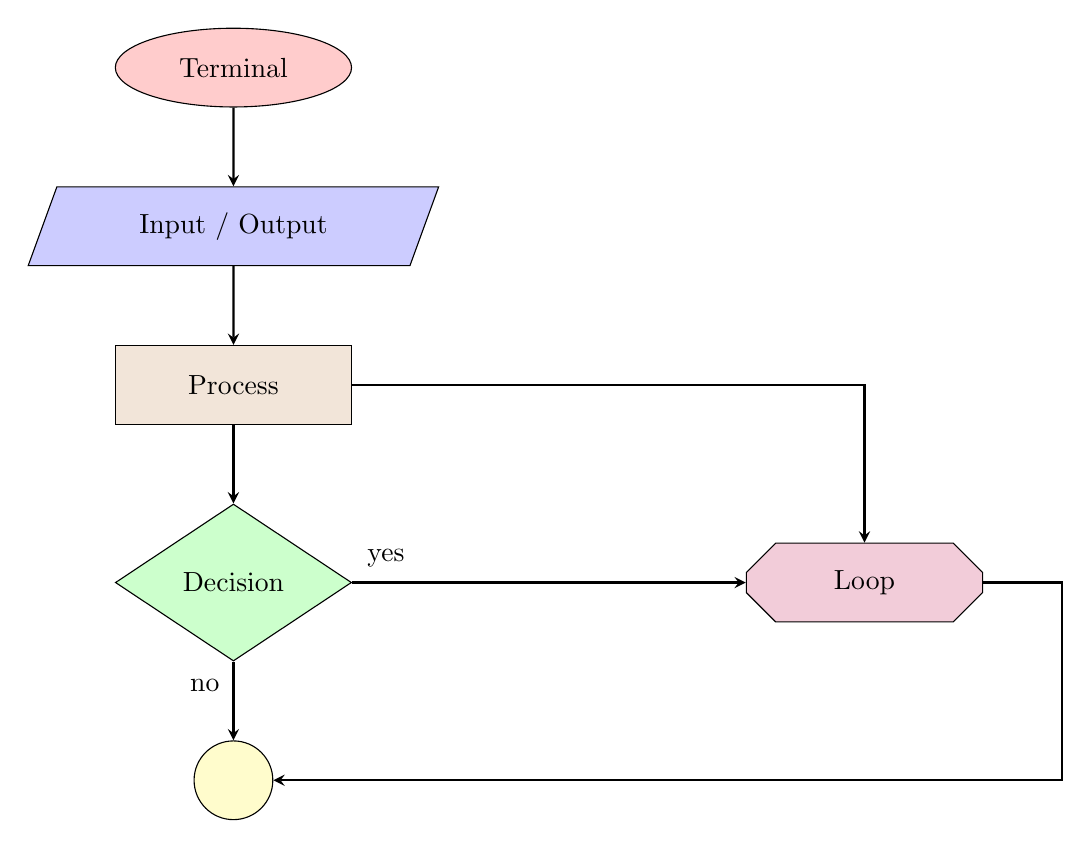
\begin{tikzpicture}[node distance=1cm]

%%% Nodes
\node[terminal] (terminal) {Terminal};
\node[io] (io) [below=of terminal] {Input / Output};
\node[process] (process) [below=of io] {Process};

\node[decision] (decision) [below=of process] {Decision};
\node[text width=1cm] (yes) [above right=1mm of decision.east] {yes};
\node[text width=1.1cm] (no) [below=1mm of decision.south] {no};

\node[junction] (junction) [below=of decision] {};
\node[loop] (loop) [right=5cm of decision] {Loop};


%%% Arrows
\draw[arrow] (terminal) -- (io);
\draw[arrow] (io) -- (process);
\draw[arrow] (process) -- (decision.north);
\draw[arrow] (decision.south) -- (junction);
\draw[arrow] (decision.east) -- (loop.west);
\draw[arrow] (loop.east) -- ++(1, 0) |- (junction.east);
\draw[arrow] (process.east) -| (loop.north);

\end{tikzpicture}

%%%%%%%%%%%%%%%%%%%%%%%%%%%%%%%%%%%%%%%%%%%%%%%%%%%%%%%%%%%%%%%%%%%%%%%%%%%%%%%
\end{document}
